\documentclass{article}

\usepackage[english]{babel} % required to compile for windows
\usepackage[utf8]{inputenc}
\usepackage[T1]{fontenc}
\usepackage{geometry}
\usepackage{listings}
\usepackage{xcolor}
\lstset{ %
	frame=single,	                   % adds a frame around the code
	numbers=none,                    % where to put the line-numbers; possible values are (none, left, right)
	numbersep=5pt,                   % how far the line-numbers are from the code
	numberstyle=\tiny\color{gray}, % the style that is used for the line-numbers
	showstringspaces=false
}
\usepackage{enumitem}
\setlist[itemize]{leftmargin=*}
\usepackage{graphicx}
\usepackage{fancyhdr} % header
\geometry{a4paper, left=2cm, right=2cm, top=3cm, bottom=4cm} 

% header
\pagestyle{fancy}
\fancyhead{} % clear header
\fancyfoot{} % clear footer
\setlength{\headheight}{50pt}

\chead{{\large Schnupperuni Informatik}}

\lhead{FOSS-AG}
\rhead{15. - 19.10.2018}
\cfoot{-\thepage-}

\begin{document}
	\begin{center}
		\huge Von Schlangen und Himbeerkuchen:\\Programmieren in der Welt von Minecraft
	\end{center}
	\section{Einführung}
		\large Schreibe ein Python-Script, das dafür sorgt, dass stets Blumen auf dem Block generiert werden, auf dem Steve sich befindet.
Gehe dafür wie folgt vor:
\begin{itemize}
	\item Binde zunächst die Minecraft-Bibliothek ein, um mit dem Spiel zu kommunizieren.
	\begin{lstlisting}[language=Python]
import mcpi.minecraft as minecraft
	\end{lstlisting}
	
	\item Baue die Verbindung zum Spiel auf.
	\begin{lstlisting}[language=Python]
mc = minecraft.Minecraft.create()
	\end{lstlisting}
	Das Objekt \textbf{mc} stellt nun die Kommunikationschnittstelle mit dem Spiel dar.
	
	\item Speichere dir die Block-ID der Blume (38) in einer Variable zwischen. Das erleichtert das Programmieren und macht den Code einfacher zu lesen.
	
	\item Verwende eine \textbf{while}-Schleife für den Hauptteil deines Scripts. Da das Platzieren der Blumen solange stattfinden soll, wie das Spiel läuft, wird eine Schleife benötigt, die nur durch Beenden des Programms abgebrochen werden kann.
	
	\item Frage innerhalb der \textbf{while}-Schleife die aktuelle Position von Steve ab. Diese benötigen wir, um an genau dieser Stelle die Blumen platzieren zu können.
	
	\item Platziere zu guter letzt an Steves aktueller Position die Blumen. 
\end{itemize}
	\section{Shuffle Block}
		\subsection{}
		\large Schreibe ein Python-Script, das dafür sorgt, dass Blöcke, die du mit der rechten Maustaste schlägst, wie unten beschrieben, durchwechseln.
Gehe dafür wie folgt vor:
\begin{itemize}
	\item Ergänze den Code nur in dem gekennzeichneten Rahmen.
	
	\item Die Liste \texttt{block\_list} beinhaltet alle Blöcke, durch die durchgewechselt werden sollen.
	
	\item Lege außerhalb der \texttt{while}-Schleife eine Variable an, die dazu dient, die aktuelle Position in \texttt{block\_list} zu speichern. Somit kannst du dir merken, welcher Block als nächstes gesetzt werden soll.
	
	\item Schreibe innerhalb der \texttt{while}-Schleife eine \texttt{for}-Schleife, die für jeden geschlagenen Block den Schleifenrumpf ausführt. Um die Liste der angeschlagenen Blöcke zu erhalten verwende die Funktion
	\begin{lstlisting}
mc.events.pollBlockHits()
	\end{lstlisting}
		
	\item Ersetze den geschlagenen Block durch den aktuellen Block in \texttt{block\_list}. Nutze dafür die Funktion
	\begin{lstlisting}
mc.setBlock(x_pos, y_pos, z_pos, block_id, 1)
	\end{lstlisting}
	Gehe danach sofort einen Schritt weiter in der Liste.
	
	\item Ist das Ende der Liste erreicht, wird die Liste wieder von vorne durchlaufen.
\end{itemize}
		\subsection{}
		Erweitere den ersten Aufgabenteil wie folgt:
\begin{itemize}
	\item Wird ein Block geschlagen, soll er nicht einfach durch den aktuellen Block in der Liste ersetzt werden, sondern abhängig vom geschlagenen Block behandelt werden. Ist der geschlagene Block nicht in der Liste vorhanden, so wird er durch den ersten Block der Liste ersetzt. Befindet sich der Block in der Liste, so wird er durch den nachfolgenden Block in der Liste ersetzt.
	
	\item Um herauszufinden, um welche Art von Block es sich handelt, kannst du die Funktion\\ \texttt{mc.getBlock(x\_pos, y\_pos, z\_pos)} verwenden.
	
	\item Hast du das Ende der Liste erreicht, fange wieder beim ersten Element an.
\end{itemize}
	\section{Lava Runner}
		\large Schreibe ein Python-Script, das einen zufälligen Parcour über das Lavabecken generiert.
\begin{itemize}
	\item Um das Lavabecken und den restlichen Rahmen zu generieren, öffne das Initiliasierungsscript \texttt{lava\_runner\_initialiser.py} und führe es aus.
	
	\item Öffne die Datei \texttt{lava\_runner.py} mit dem Editor. Diese Datei enthält bereits Code und muss lediglich im gekennzeichneten Bereich erweitert werden.
	
	\item Die Funktion \texttt{generate\_parcour} bekommt die Koordinaten (\texttt{x, y, z}) übergeben. Die Koordinaten geben die Position des Blocks an auf dem ihr steht, wenn du \texttt{lava\_runner.py} ausführst. Ausgehend von dieser Position soll der zufällige Parcour über das Lavabecken gebaut werden.
	
	\item Außerhalb von \texttt{generate\_parcour} gibt es zwei Variablen \texttt{x\_boundary} und \texttt{z\_boundary}. Diese geben den Rand der Arena an.
	
	\item In \texttt{generate\_parcour}: Schreibe eine Schleife, die solange läuft, wie \texttt{x} und \texttt{z} nicht den Rand der Arena überschreiten.
	
	\item  Setze mit \texttt{setBlock(x, y, z, block.ICE)} den nächsten Block des zufälligen Parcours.
	
	\item Als nächstes muss die Position für den nächsten Block bestimmt werden. Mit Hilfe der Funktion \texttt{random.randint(unter\_grenze, obere\_grenze)} kannst du dir einen zufälligen Wert zwischen den angegeben Grenzen geben lassen. Überlege wie die neuen Werte \texttt{x2, y2} und \texttt{z2} aussehen könnten und wähle die Grenzen \texttt{untere\_grenze, obere\_grenze} demnentsprechend. Achte darauf, dass man den neuen Block mit einem Sprung vom vorherigen Block aus erreichen können muss. Du kannst dafür die Abbildung weiter unten zur Hilfe nehmen.
	
	\item Ist die neue Position \texttt{(x2, y2, z2)} vom vorherigen Block aus erreichbar, überschreibe \texttt{(x, y, z)} mit \texttt{(x2, y2, z2)}. Ist die neue Position allerdings nicht erreichbar, dann kannst du mit dem Schlüsselwort \texttt{continue} dafür sorgen, dass neue Werte für \texttt{x2, y2} und \texttt{z2} ausgewählt werden.

\end{itemize}
\begin{figure}
\centering
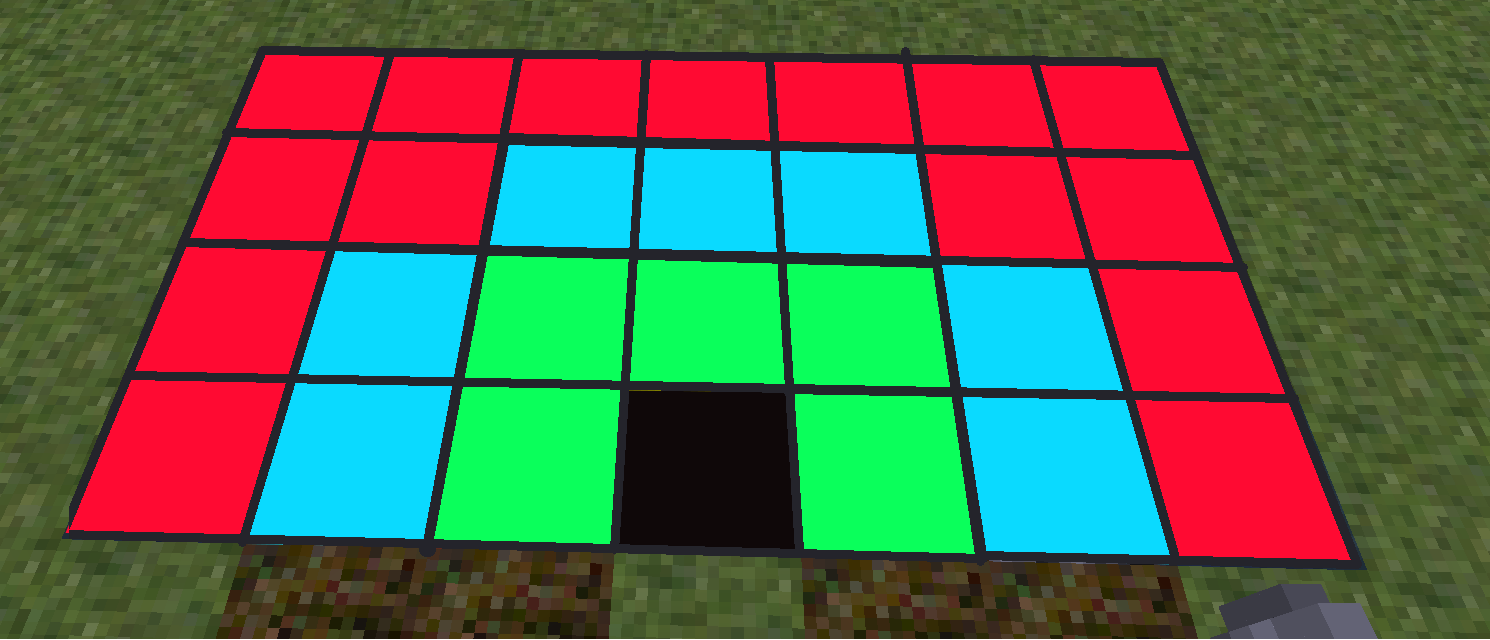
\includegraphics[scale=0.25]{src/lava_runner/res/1layer.png}
\caption{Das schwarz markierte Feld stellt die Position des vorherigen Blocks dar, die roten Felder sind nicht erreichbar, weshalb ein Block verworfen werden soll, falls er zufällig auf diesem Feld platziert werden soll.}
\end{figure}

	\newpage
	\section{Astroid}
		\textbf{\large Raumfahrer Training 101:}\\
Du bist mit deinem Raumschiff mitten im Weltall unterwegs. Bereit neue Planeten zu entdecken. Doch irgendwo im Andromeda-Nebel versagen deine Motoren. Niemand weit und breit, der dich zum nächsten Planeten bringen kann. Nicht mal Asteroiden sind zu sehen.\\\\
\textbf{Schritt 1: Asteroiden erscheinen lassen}\\
Versuche zuerst die Asteroiden erscheinen zu lassen, dann ist es im Weltraum nicht mehr so leer.
\begin{itemize}
	\item Prüfe ob der Asteroiden Timer (\texttt{state.astroid\_timer}) abgelaufen ist
	\begin{itemize}
		\item \texttt{state.astroid\_timer == 0}
	\end{itemize}
	\item Ist dieser abgelaufen, erzeuge einen Asteroiden mithilfe des Befehles \texttt{Astroid.create\_astroid()}
	\item Setze den \texttt{state.astroid\_timer} neu, auf den Wert \textbf{100 - (astroids\_faster * 2)}. Nutze dafür die Funktion \texttt{state.set\_astroid\_timer(t)}
	\item Ändere den Wert von \texttt{state.astroids\_faster}
	\begin{itemize}
		\item Gilt \texttt{state.astroids\_faster} $\geq$ 35, dann setze den Wert wieder auf 35
		\item ansonsten erhöhe den Wert von \texttt{state.astroid\_timer} um 5
		\item Dafür steht die Funktion \texttt{state.set\_astroids\_faster(af)} zur Verfügung.
	\end{itemize}
\end{itemize}
\textbf{Schritt 2: Kollisionen}\\
Jetzt sind wieder viele Asteroiden unterwegs, aber ohne Kollisionen ist das Ganze langweilig.
\begin{itemize}
	\item Überprüfe mithilfe des Befehls \texttt{player\_astroid\_collision\_check(astroid, astroid\_rect, player\_rect)} ob eine Kollision vorliegt.
	\item Ist das der Fall unterscheide 2 Fälle:
	\begin{itemize}
		\item Hat der Spieler noch Leben, dann verringere die Lebensanzahl
		\item Ansonsten beende das Spiel, in dem du die Funktion \texttt{state.set\_done()} aufrufst.
	\end{itemize}
\end{itemize}
\textbf{Schritt 3: Asteroiden treffen}\\
Nun kommen Asteroiden auf dich zu, aber die Zielsysteme funktionieren scheinbar nicht. Keiner der Schüsse scheint zu treffen.
\begin{itemize}
	\item Für jeden Schuss in der Liste \texttt{state.shots} muss geguckt werden ob der aktuelle Asteroid getroffen wurde.
	\begin{itemize}
		\item Speichere die Ausmaße des aktuellen Asteroiden in der Variablen \texttt{bullet\_rect} ab. Die Ausmaße bekommst du durch den Befehl \texttt{bullet.get\_rect\_bullet()}
		\item Überprüfe mit dem Befehl \texttt{check\_bullet\_astroid\_hit(bullet, bullet\_rect, astroid\_rect)} ob der Asteroid getroffen wurde.
		\begin{itemize}
			\item Wurde der Asteroid getroffen, dann erhöhe den Wert von Zähler für die Treffer um 1 (\texttt{state.increment\_num\_hits()})
			\item Überprüfe, ob der Wert \texttt{astroid.hit\_count} gleich 1 ist.
			\begin{itemize}
				\item Gilt dies, dann entferne den Asteroiden mit \texttt{state.remove\_astroid(astroid)}.
				\item Ansonsten erhöhe den Zähler für die Treffer mit \texttt{astroid.increment\_hit\_count()}.
			\end{itemize}
		\end{itemize}
	\end{itemize}
\end{itemize}
\textbf{Schritt 4: Bewegen}\\
Nun bewegen wir uns wieder durch das Weltall, aber wie sollen wir zu unserem Ziel kommen, wenn wir nicht ausweichen können?
\begin{itemize}
	\item Überlege dir Tasten mit denen du das Raumschiff steuern willst.
	\item Finde heraus welche Taste gedrückt wurde
	\begin{itemize}
		\item \texttt{pressed = pygame.key.get\_pressed()}
		\item \texttt{if pressed[pygame.K\_DOWN]} (Pfeiltaste nach unten)
	\end{itemize}
	\item Schreibe eine if-Bedingung für jede Bewegungstaste
	\item Bewege den Spieler mit player.move(x, y)
	\begin{itemize}
		\item \texttt{x} ist verantwortlich für einen Flug nach links oder rechts
		\item \texttt{y} ist verantwortlich für einen Flug nach oben oder unten
		\item Verändere den Wert um den Wert der Variablen \texttt{player\_speed}
		\item Soll nur einer der beiden Werte verändert werden, setze den anderen Wert auf 0.
	\end{itemize}	 
\end{itemize}
	\newpage
	\section{Snake}
		\textbf{\large Snake:}\\
Du findest eine hungrige Schlange, die fast verhungert ist. Hilf ihr die Äpfel einzusammeln und wieder zu Kräften zu kommen.\\\\
\textbf{Schritt 1: Durchgehendes Füttern}\\
Zunächst brauchen wir eine Schleife, die erst dann abbricht, wenn das Spiel entgültig vorbei ist. Und eine Schleife, die überprüft, ob das GameOver erreicht ist.
\begin{itemize}
	\item Benutze für die erste while-Schleife als Bedingung die Negation von der Variablen \textit{done}. Alle weiteren Schritte werden in dieser Schleife benötigt
	\item Die zweite Schleife soll so lange laufen, bis der Wert der Variablen \textit{gameOver} nicht mehr gleich \textbf{True} ist
	\item In der zweiten Schleife soll nun die Funktion \textit{show\_end\_screen(snake\_length)} aufgerufen werden um das Game Over anzuzeigen
\end{itemize}
Nach Schritt 1 könnt ihr bereits euer Spiel zum ersten mal starten.\\
\textbf{Schritt 2: Bewegen}\\
Jetzt seht ihr die Welt in der sich die Schlange befinden wird, allerdings ist die Schlange noch nicht zu sehen. Allerdings solltest du dich erst mal um die Steuerung der Schlange kümmern.
\begin{itemize}
	\item Benutze als erstes die Funktion \textit{get\_pressed\_button()} um die aktuell benutzte Taste zu erhalten. Die Funktion wird allerdings zwei Werte zurück geben. Zum einen den Typ des Tastendruckes und die Art der Taste.
	\begin{itemize}
		\item Bsp.: e\_type, e\_key = get\_pressed\_button()
	\end{itemize}
	\item prüfe nun ob die Variable \textit{e\_type} nicht \textbf{None} entspricht.
	\item Ist das der Fall sind zwei Fälle zu unterscheiden
	\begin{itemize}
		\item[1] \textit{e\_type} ist gleich \textbf{pygame.QUIT}, dann muss \textit{done} auf \textbf{True} gesetzt werden
		\item[2] \textit{e\_type} ist gleich \textbf{pygame.KEYDOWN}, dann müssen diese Fälle für die Variable \textit{e\_key} unterschieden werden
		\begin{itemize}
			\item Ist \textit{e\_key} gleich \textbf{pygame.K\_Left} und \textit{snake\_x\_change} $\leq$ \textbf{0} muss \textit{snake\_x\_change} auf \textbf{$-$ \textit{block\_size}} und \textit{snake\_y\_change} auf \textbf{0} gesetzt werden
			\item Ist \textit{e\_key} gleich \textbf{pygame.K\_RIGHTt} und \textit{snake\_x\_change} $\geq$ \textbf{0} muss \textit{snake\_x\_change} auf \textbf{\textit{block\_size}} und \textit{snake\_y\_change} auf \textbf{0} gesetzt werden
			\item Ist \textit{e\_key} gleich \textbf{pygame.K\_UP} und \textit{snake\_y\_change} $\leq$ \textbf{0} muss \textit{snake\_y\_change} auf \textbf{$-$ \textit{block\_size}} und \textit{snake\_x\_change} auf \textbf{0} gesetzt werden
			\item Ist \textit{e\_key} gleich \textbf{pygame.K\_DOWN} und \textit{snake\_y\_change} $\geq$ \textbf{0} muss \textit{snake\_y\_change} auf \textbf{\textit{block\_size}} und \textit{snake\_x\_change} auf \textbf{0} gesetzt werden
		\end{itemize}
	\end{itemize}
\end{itemize}
\textbf{Schritt 3: Apfel und Schlange}\\
Jetzt wo die Steuerung fertig ist, brauchen wir noch die Schlange und den Apfel.
\begin{itemize}
	\item Als erstes wird der Apfel gezeichnet. Benutze dazu den Befehl \textit{draw\_apple(apple\_x, apple\_y)}
	\item Nun müssen die Werte von \textit{snake\_x} und \textit{snake\_y} um den entsprechenden Wert \textit{snake\_x\_change} bzw. \textit{snake\_y\_change} erhöht werden
	\item Lege eine Variable \textit{snake\_segment} an und speichere in dieser \textbf{[\textit{snake\_x}, \textit{snake\_y}]} ab
	\item Füge diese neu erstellte Liste der Liste \textit{snake\_list} durch dem Befehl \textit{append} hinzu
	\item Prüfe nun ob die Schlange die bisher erlaubte Länge überschritten hat (Tipp: len(snake\_list) > snake\_length)
	\begin{itemize}
		\item Ist das der Fall lösche das erste Element der Liste mit dem Befehl \textit{del snake\_list[0]}
	\end{itemize}
	\item Speichere den Wert, der durch den Befehl \textit{snake\_bit(snake\_list, snake\_segment) or snake\_left\_screen(snake\_x, snake\_y)} erzeugt wird, in der Variablen \textit{gameOver} ab
	\item Nun muss nur noch die Schlange durch den Befehl \textit{snake(block\_list, snake\_list)} erzeugt werden
\end{itemize}
\textbf{Schritt 4: Essen}\\
Jetzt ist die Schlange wieder unterwegs und zu sehen, allerdings kann sie noch nichts essen.
\begin{itemize}
	\item Prüfe ob \textit{snake\_x} = = \textit{apple\_x} \textbf{und} \textit{snake\_y} = = \textit{apple\_y}
	\begin{itemize}
		\item Jetzt brauchst du eine neue Position für den Apfel. Hole dir mit den Befehlen \textit{get\_new\_apple\_x()} und \textit{get\_new\_apple\_y()} neue x und y Werte und speichere diese in die entsprechenden Variablen \textit{apple\_x} bzw. \textit{apple\_y}
		\item Zum Schluss muss nur noch die zulässige Länge der Schlange \textit{snake\_lenght} erhöht werden
	\end{itemize}	 
\end{itemize}
\end{document}